\begin{center}
\Huge{Supplementary Information}
\vspace{5cm}
\end{center}

\section{Topologically Diverse (TD) Dataset}
The RTP dataset is described in detail in the main text. All porous structures used in this study—including the RTP, TD, and ATTD datasets—are openly available in the dedicated repository associated with this paper: \url{https://github.com/dioscuri-tda/direction-aware-tda-for-porous-materials}. 
The repository also provides a utility for converting the voxelized data into VTK format, enabling straightforward visualization and rendering using standard tools such as ParaView.

\subsection{Generation of porous structures}
\subsubsection{Random Voronoi structures}\label{app:voronois}

600 random Voronoi structures were generated. For each structure, between 3 and 12 points were sampled from a unit cell (randomly, uniform distribution), with the space between them tesselated into Voronoi regions and the edges between regions used as a skeleton for the structure. The voxels traversed by the edges are approximated using the Bresenham's Line Algorithm~\cite{bresenham1965algorithm} and included within the structure. The edges are thickened to form struts with a square-shaped cross-section, with the side length of the square randomly drawn from the uniform distribution between 0.06 and 0.14. In order to guarantee periodicity of the structure, copies of the original points are generated in cells neighbouring the unit cell as well and the Voronoi tesselation of space, voxelisation of edges and subsequent thickening is conducted within the neighbouring cells as well (see Fig. \ref{fig:voronoi} for a visualization of a 2D version of the procedure), with the neighboring cells discarded at the last stage of the procedure. 

\begin{figure}[h!]
    \centering
    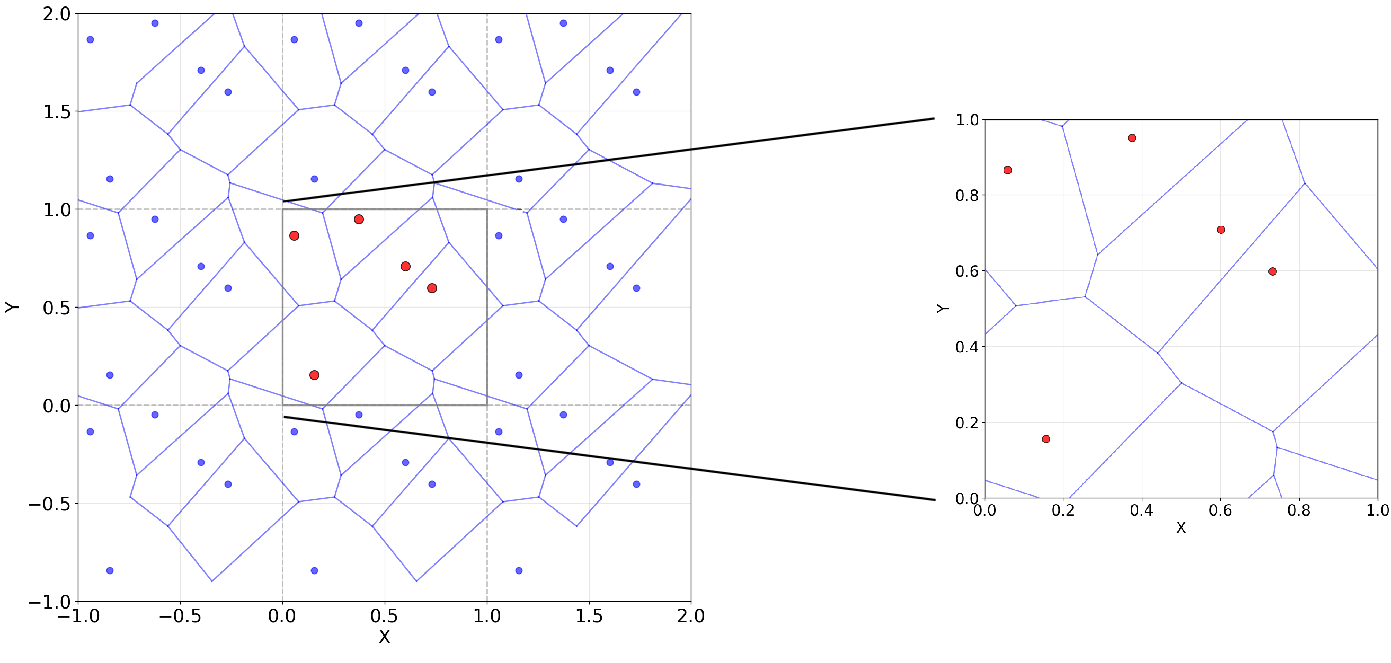
\includegraphics[width=0.89\linewidth]{Voronoi.png}
    \caption{A 2D visualisation of the algorithm for generating random Voronoi structures satisfying periodic boundary conditions.}
    \label{fig:voronoi}
\end{figure}

\subsubsection{Zeolites}\label{sec:zeolites}

More than 3000 predicted zeolitic structures were recovered from Michael Deem's database~\cite{C0CP02255A, deem2023pcod}. Each structure is described by the basis cell vector and the locations of Si and O atoms in a unit cell. We restricted the studies to structures with a perpendicular shape of the unit cell, which still left over 1500 structures. We transformed the structures from perpendicular to the normalized $1\times1\times1$ cubic volume by stretching/compression. We thickened the edges by dilation to form struts with a square-shaped cross-section of side length 0.12. We used 300 randomly drawn structures from the dataset and connected the locations of the Si atoms in these structures after the stretching/compression to the locations of their nearest Si neighbors (O atoms were not used in the structure). The connections formed the skeleton of the structure. Periodic boundary conditions were guaranteed by a procedure similar to the one used for random Voronoi structures, involving generating copies of the original Si atom locations in cells neighbouring the unit cell and connecting them to their nearest neighbours as well. Another 299 structures were created on the basis of different randomly drawn structures from using Michael Deem's database~\cite{C0CP02255A, deem2023pcod} using the same algorithm, but with using 0.04 instead of 0.12 as the side length of the square-shaped cross-section of the struts.  
This gives a total of 580 zeolite structures.  %599

\subsubsection{Diamond structures}

299 diamond-resembling structures were generated. Each structure was generated by creating within the unit cell 8 vertices corresponding to atoms in a diamond lattice and creating between the vertices edges corresponding to bonds between the atoms. The precise locations of the vertices were determined by adding a stochastic displacement to the location of the corresponding atom in the diamond lattice. Each of the three-dimensional components of the stochastic displacement for all vertices in a given lattice were drawn from a normal distribution with a standard deviation $\epsilon$ itself drawn from a uniform distribution between 0 and 0.1 (compare to 1.0 being the length of the side of a unit cell). That way, the amount of stochasticity was varied between the structures. The edges connecting the vertices were thickened via dilation to form struts with square-shaped cross-sections, with the length of the side of the cross-section drawn from a uniform distribution between 0.06 and 0.26. That way, the volume fraction was varied between structures.

\subsubsection{Cubic structures}

300 structures resembling a simple cubic strut were generated using the procedure used for diamond structures, with the only difference the 8 initiating points are not the locations of atoms in a diamond structures like in the former dataset, but instead the following set of points: [0, 0, 0],
        [0.5, 0, 0],
        [0, 0.5, 0],
        [0, 0, 0.5],
        [0, 0.5, 0.5],
        [0.5, 0, 0.5],
        [0.5, 0.5, 0],
        [0.5, 0.5, 0.5]. Replicating further steps from the procedure used to generate the diamond-like structures leads to structures resembling a classical cubic strut, with varying thicknesses of the struts and levels of randomization in locations of the struts' vertices. 


\subsubsection{Splines}

To generate a family of smooth porous morphologies, we construct a random \emph{periodic} scalar field on the unit cell and then threshold it.
Let $n=\texttt{sampling}$ be the number of spline control points per direction and draw i.i.d.\ coefficients
\begin{equation}
r_{ijk}\sim\mathcal U(0,1),\qquad i,j,k=1,\dots,n .
\end{equation}
In \textsc{Mathematica}, the command
\texttt{BSplineFunction} builds a trivariate tensor-product B-spline field
(with \texttt{SplineDegree->3}, \texttt{SplineClosed->True}, \texttt{SplineKnots->"Unclamped"}), i.e.
\begin{equation}
f(x,y,z)=\sum_{i=1}^{n}\sum_{j=1}^{n}\sum_{k=1}^{n}
r_{ijk}\,N_{i,3}(x)\,N_{j,3}(y)\,N_{k,3}(z),
\label{eq:spline_field}
\end{equation}
where $\{N_{i,3}\}$ are cubic B-spline basis functions (defined via the Cox--de Boor recursion), and the ``closed'' setting enforces periodicity across the cell boundaries \cite{deBoor1978,wolframBSplineFunction}.

A binary structure is then obtained as a super-level set. Using wrapped (periodic) coordinates
$\tilde{\boldsymbol{x}}=(x\bmod 1,\,y\bmod 1,\,z\bmod 1)$ (implemented with \texttt{Mod}), we voxelize on an $L\times L\times L$ grid (here $L=80$) by
\begin{equation}
T_{abc}(t)=\mathbf{1}\Bigl\{\,f\!\bigl(\tfrac{a}{L},\tfrac{b}{L},\tfrac{c}{L}\bigr)\ge t\,\Bigr\},
\qquad a,b,c=0,\dots,L-1,
\label{eq:thresholding}
\end{equation}
and report the volume fraction
\begin{equation}
\phi(t)=\frac{1}{L^{3}}\sum_{a,b,c} T_{abc}(t).
\end{equation}
Varying the threshold $t$ (in our implementation, on an approximately uniform grid in $[0.35,0.50]$) produces two independent subsets of spline-based structures each, spanning a range of $\phi(t)$ while preserving smoothness and periodic tiling of the unit cell.
Total of 596 spline structures were used in the dataset.

\section{Results for RTPxyz dataset}
\begin{figure}
    \centering
    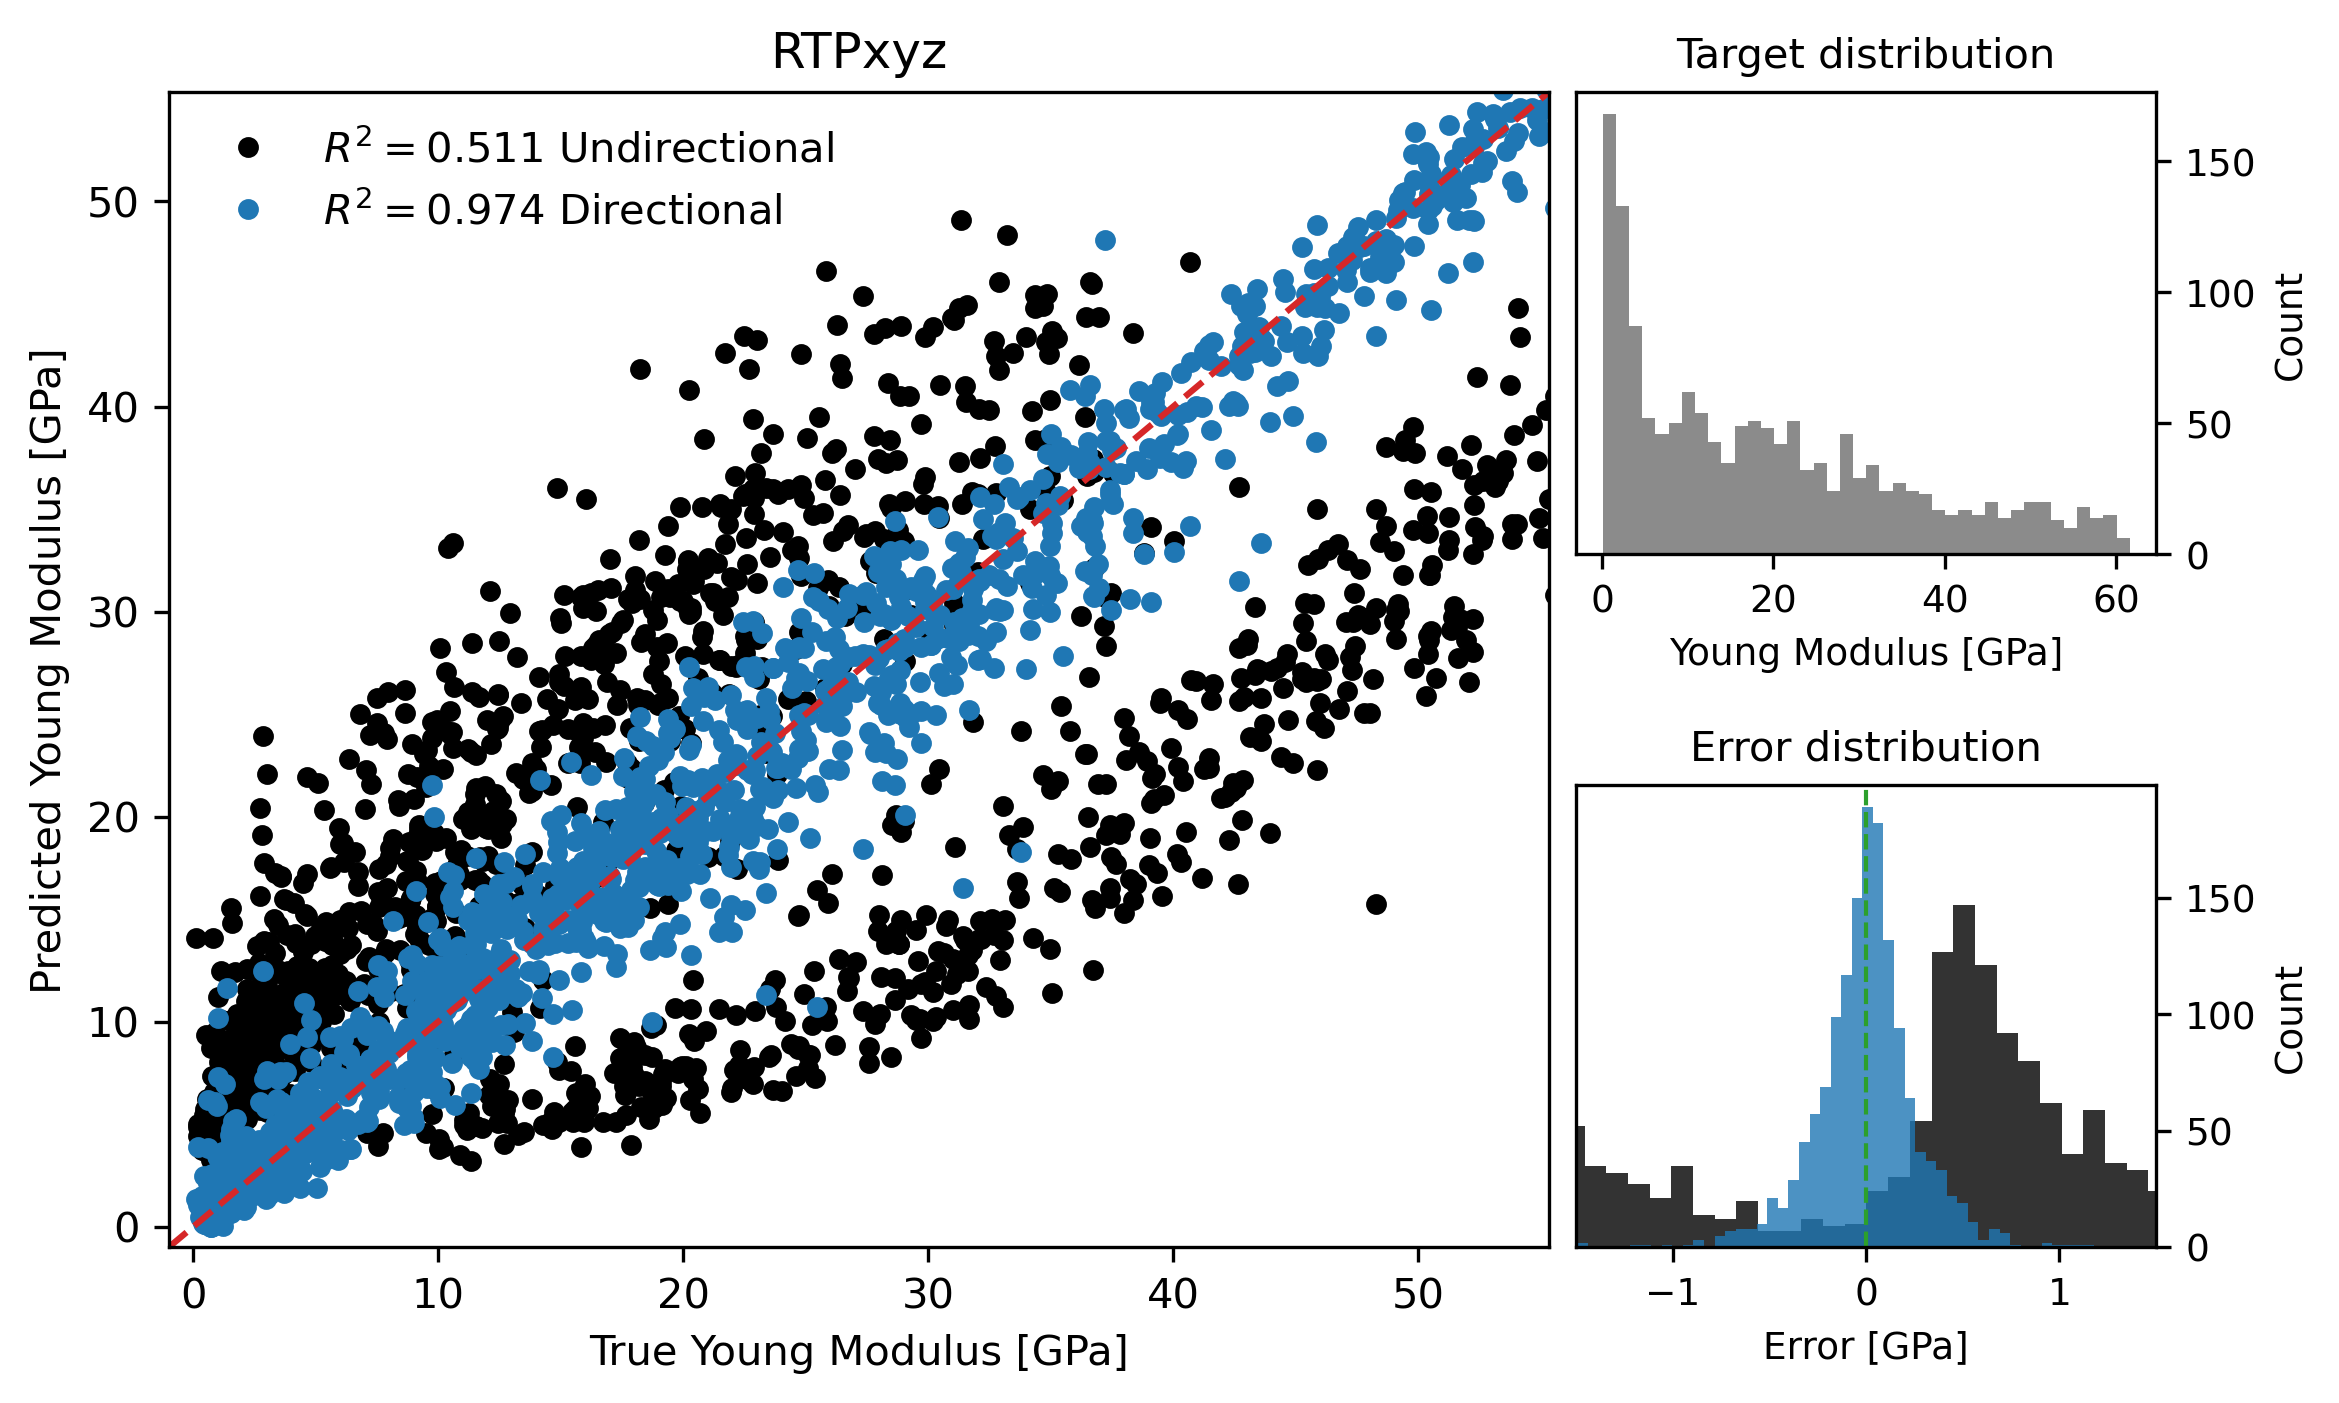
\includegraphics[width=0.75\textwidth]{scatter_rtp_xyz.png}
    \caption{Predicted versus FFTMAD-computed Young’s modulus for the RTPxyz dataset. The same as Figure 4 in the Manuscript but for the RTPxyz dataset. }
    \label{fig:scatter_rtp_xyz}
\end{figure} 

Models were additionally trained on the RTPxyz dataset, which aggregates Young’s modulus values computed for the RTP structures along all three Cartesian directions. This dataset comprises a total of 1500 samples, of which two thirds correspond to the mechanically easy axes ($x$ and $y$) and one third to the mechanically hard axis ($z$). The scatter plot of predicted versus FFTMAD-computed Young’s modulus for models trained with directional and non-directional descriptors is shown in Fig.~\ref{fig:scatter_rtp_xyz}, while the corresponding regression metrics are summarized in Table~\ref{tab:metrics_rtp_xyz}.

Models based on directional descriptors maintain high predictive accuracy, with predictions tightly clustered around the diagonal and a coefficient of determination of $R^2 = 0.974$. In contrast, models relying on non-directional descriptors perform poorly, achieving only $R^2 = 0.511$. The corresponding scatter plot reveals a pronounced bifurcation: predictions obtained from non-directional descriptors split into two distinct branches, one above and one below the diagonal.

\begin{table}[]
\centering
\caption{Cross-validated regression metrics for Young’s modulus prediction using CatBoost with PH, ECP, and PH+ECP topological summaries, and a CNN baseline trained directly on voxelized structures. Reported as average over 8 folds. The same as Table~1 in the manuscript but for the RTPxyz dataset.}
\label{tab:metrics_rtp_xyz}
\begin{tabular}{lcc|cc||l|rrrr}
\hline 
 & \multicolumn{2}{l}{} & \multicolumn{2}{|l||}{CNN baseline} &  & \multicolumn{2}{l}{Non-directional} & \multicolumn{2}{l}{Directional} \\
Dataset & $\sigma(k)$ & $\sigma(L)$ & $R^2$ & MAE & Method & $R^2$ & MAE & $R^2$ & MAE \\ \hline
RTPxyz & 0.38 & 1.77 & 0.990 & 1.88 & PH     & 0.509 & 13.26 & 0.548 & 13.61 \\
 &  &  &  &                        & ECP    & 0.493 & 15.11 & 0.974 & 3.09 \\
 &  &  &  &                        & PH+ECP & 0.511 & 9.94  & 0.974 & 2.89 \\ \hline
\end{tabular}
\end{table}


The upper branch (systematic overestimation) predominantly contains data points corresponding to compression along the mechanically easy $x$ and $y$ axes, where the true Young’s modulus is relatively low. The lower branch (systematic underestimation) consists mainly of samples compressed along the mechanically hard $z$ axis, where the true Young’s modulus is significantly higher. This clear separation demonstrates that non-directional descriptors fail to encode the loading direction and therefore cannot distinguish between mechanically inequivalent orientations of the same structure.

Only a small fraction of predictions obtained with non-directional descriptors lie close to the line of perfect agreement, which is reflected in the broadened and multimodal error distribution shown in the inset histogram. In contrast, no such branching behavior is observed for directional descriptors: predictions remain symmetrically distributed around the diagonal, indicating that direction-aware topology provides a consistent and physically meaningful representation of anisotropic mechanical response.

\section{Per-Fold Cross-Validation Performance}
The implemented cross-validation procedure allows for a direct comparison of the models within each fold, as identical train/validation/test splits are used throughout. This provides substantially more detailed insight than the averaged results reported in Table 1 of the manuscript.

The per-fold results for the $R^2$ and MAE metrics are presented in Tables~\ref{tab:fold_r2} and~\ref{tab:fold_mae}, respectively. The column Gain indicates whether the use of directional descriptors improves the performance, i.e., increases $R^2$ or decreases MAE. The last two rows of each table report the mean and standard deviation across folds for each method.

We report results for the PH+ECP descriptor on the RTPxz and RTPxy datasets, as this combination constitutes the main result of the paper. As shown in the tables, the improvement obtained by incorporating directional descriptors is consistent across all folds and for both datasets: $R^2$ increases and MAE decreases in every single split, demonstrating that the performance gain is systematic rather than incidental. The only exception is the standard deviation of $R^2$ for RTPxy, which is slightly higher for the directional descriptors compared to the non-directional variant.

\begin{table}[]
\caption{$R^2$ scores obtained in each cross-validation fold for the RTPxz and RTPxy datasets using the PH+ECP descriptor. Results for the CNN model are provided for reference. The column \textit{Gain} indicates whether the inclusion of directional descriptors improves performance (i.e., increases $R^2$). The last two rows report the mean and standard deviation across folds.}
\label{tab:fold_r2}
\begin{tabular}{r|rrlr|rrlrr}
\hline
\multicolumn{1}{l|}{$R^2$} & \multicolumn{4}{c|}{RTPxz} & \multicolumn{4}{c}{RTPxy} & \multicolumn{1}{l}{} \\
\multicolumn{1}{l|}{} & \multicolumn{3}{c}{PH+ECP} & \multicolumn{1}{l|}{CNN} & \multicolumn{3}{c}{PH+ECP} & \multicolumn{1}{l}{CNN} & \multicolumn{1}{l}{} \\
\multicolumn{1}{l|}{fold} & \multicolumn{1}{l}{Directional} & \multicolumn{1}{l}{Non-directional} & Gain & \multicolumn{1}{l|}{---} & \multicolumn{1}{l}{Directional} & \multicolumn{1}{l}{Non-directional} & Gain & \multicolumn{1}{l}{--} &  \\ \hline
1 & 0.9706 & 0.7213 & Yes & 0.9689 & 0.9176 & 0.9012 & Yes & 0.9852 &  \\
2 & 0.9829 & 0.8088 & Yes & 0.9876 & 0.9777 & 0.9587 & Yes & 0.9751 &  \\
3 & 0.9814 & 0.7638 & Yes & 0.9923 & 0.9265 & 0.9179 & Yes & 0.9889 &  \\
4 & 0.9726 & 0.7582 & Yes & 0.9899 & 0.9132 & 0.9013 & Yes & 0.9823 &  \\
5 & 0.9795 & 0.7018 & Yes & 0.9889 & 0.9408 & 0.9162 & Yes & 0.9892 &  \\
6 & 0.9798 & 0.7473 & Yes & 0.9776 & 0.9525 & 0.9035 & Yes & 0.9732 &  \\
7 & 0.9764 & 0.7866 & Yes & 0.9828 & 0.9532 & 0.9130 & Yes & 0.9863 &  \\
8 & 0.9816 & 0.7464 & Yes & 0.9884 & 0.9233 & 0.9169 & Yes & 0.9541 &  \\ \hline
\multicolumn{1}{l|}{Mean} & 0.9781 & 0.7543 & Yes & 0.9846 & 0.9381 & 0.9161 & Yes & 0.9793 &  \\
\multicolumn{1}{l|}{Std} & 0.0045 & 0.0340 & Yes & 0.0078 & 0.0221 & 0.0186 & No & 0.0118 &  \\ \hline
\end{tabular}
\end{table}

\begin{table}[]
\caption{The same as Table \ref{tab:fold_r2} but for MAE.}
\label{tab:fold_mae}
\begin{tabular}{r|rrlr|rrlrr}
\hline
\multicolumn{1}{l|}{MAE} & \multicolumn{4}{c|}{RTPxz} & \multicolumn{4}{c}{RTPxy} & \multicolumn{1}{l}{} \\
\multicolumn{1}{l|}{} & \multicolumn{3}{c}{PH+ECP} & \multicolumn{1}{l|}{CNN} & \multicolumn{3}{c}{PH+ECP} & \multicolumn{1}{l}{CNN} & \multicolumn{1}{l}{} \\
\multicolumn{1}{l|}{fold} & \multicolumn{1}{l}{Directional} & \multicolumn{1}{l}{Non-directional} & Gain & \multicolumn{1}{l|}{---} & \multicolumn{1}{l}{Directional} & \multicolumn{1}{l}{Non-directional} & Gain & \multicolumn{1}{l}{--} &  \\ \hline
1 & 2.116 & 7.532 & Yes & 2.269 & 2.051 & 2.202 & Yes & 0.871 &  \\
2 & 1.572 & 6.511 & Yes & 1.504 & 1.120 & 1.493 & Yes & 1.225 &  \\
3 & 1.631 & 6.803 & Yes & 1.185 & 1.512 & 1.763 & Yes & 0.701 &  \\
4 & 1.965 & 6.757 & Yes & 1.203 & 1.674 & 1.735 & Yes & 0.792 &  \\
5 & 1.820 & 7.821 & Yes & 1.380 & 1.764 & 2.087 & Yes & 0.735 &  \\
6 & 1.891 & 7.331 & Yes & 2.062 & 1.656 & 2.213 & Yes & 1.243 &  \\
7 & 2.119 & 6.788 & Yes & 2.021 & 1.850 & 2.396 & Yes & 1.060 &  \\
8 & 1.730 & 6.878 & Yes & 1.336 & 1.906 & 1.989 & Yes & 1.520 &  \\ \hline
\multicolumn{1}{l|}{Mean} & 1.855 & 7.053 & Yes & 1.620 & 1.692 & 1.985 & Yes & 1.018 &  \\
\multicolumn{1}{l|}{Std} & 0.207 & 0.454 & Yes & 0.430 & 0.284 & 0.300 & Yes & 0.293 &  \\ \hline
\end{tabular}
\end{table}

% \bibliographystyle{sn-mathphys-num}
% \bibliography{references}



